\documentclass[a4paper, 12pt]{article}
\usepackage[top=1.8cm, bottom=1.8cm, left=1.5cm, right=1.5cm]{geometry}
\usepackage{float}
\usepackage[utf8]{inputenc}
\usepackage{pgfplots}
\pgfplotsset{width=10cm, compat=1.18}



\begin{document}
	
	\begin{center}
		Universidade Federal do Rio Grande do Norte
		
		Departamento de Engenharia da Computação e Automação  
		
		DCA3703 - Programação Paralela  
		
		\textbf{Tarefa 15: Difusão de calor usando MPI}  
		
		\textbf{Aluno:} Daniel Bruno Trindade da Silva  
	\end{center}  
	
	\section{Introdução}
	
	\hspace{0.62cm}Este relatório tem como objetivo apresentar os conhecimentos adquiridos durante a realização da Tarefa 15 da disciplina de \textbf{Programação Paralela}. A atividade teve como objetivo mensurar o tempo de comunicação entre os processos usando ferramentas do MPI. Para isso será realizada a implementação e análise de um programa que simulasse a difusão de calor em uma barra 1D. 
	
	\section{Enunciado}
	
	\hspace{0.62cm}Implemente uma simulação da difusão de calor em uma barra 1D, dividida entre dois ou mais processos MPI. Cada processo deve simular um trecho da barra com células extras para troca de bordas com vizinhos. Implemente três versões: uma com \texttt{MPI\_Send/MPI\_Recv}, outra com \texttt{MPI\_Isend/ MPI\_Irecv} e \texttt{MPI\_Wait}, e uma terceira usando \texttt{MPI\_Test} para atualizar os pontos internos enquanto aguarda a comunicação. Compare os tempos de execução e discuta os ganhos com sobreposição de comunicação e computação.
	
	\section{Desenvolvimento}
	\hspace{0.62cm}Para atender aos requisitos da atividade, foram desenvolvidas três versões de um programa em C com MPI para simular a difusão de calor unidimensional. 
	
	Em todas as implementações, a barra 1D de tamanho $N$ é dividida entre os $P$ processos MPI, onde cada processo é responsável por calcular a temperatura de um segmento de $N/P$ células. Para permitir a troca de informações de contorno com os processos vizinhos, cada processo aloca duas células extras (ghost cells), uma no início e outra no fim de seu subdomínio local. A inicialização da barra atribui um valor de temperatura elevado a uma célula central da barra global e zero às demais. As condições de contorno globais da barra são fixas em 0.0. O tempo de execução de cada simulação é medido utilizando \texttt{MPI\_Wtime()} e o tempo máximo entre todos os processos é obtido com \texttt{MPI\_Reduce}.
	
	As três versões implementadas diferem na forma como a comunicação das células de borda é realizada da seguinte forma:
	
	\begin{itemize}
		\item \textbf{Versão 1:} - Nesta implementação, a troca de dados das células de borda é realizada utilizando as funções bloqueantes \texttt{MPI\_Send} e \texttt{MPI\_Recv}. A natureza bloqueante dessas chamadas implica que um processo pode ficar ocioso enquanto espera a conclusão de uma operação de envio ou recebimento.
		
		\item \textbf{Versão 2:} - A segunda implementação utiliza as versões não bloqueantes das chamadas de comunicação, \texttt{MPI\_Isend} e \texttt{MPI\_Irecv}, para a troca das células de borda. Após iniciar todas as operações de comunicação necessárias, a função \texttt{MPI\_Waitall} é chamada. Esta função bloqueia o processo até que todas as comunicações não bloqueantes (tanto envios quanto recebimentos) especificadas sejam concluídas. Somente após o retorno de \texttt{MPI\_Waitall}, o cálculo da nova temperatura para todas as células locais é efetuado. Nesta abordagem, embora as operações sejam não bloqueantes, a computação dos pontos da malha só ocorre após a finalização de toda a comunicação.
		
		\item \textbf{Versão 3 (mpi\_test.c):} - Esta terceira versão também emprega chamadas de comunicação não bloqueantes, \texttt{MPI\_Isend} e \texttt{MPI\_Irecv}, para a troca de dados das células de borda. No entanto, adota uma estratégia para tentar sobrepor o cálculo com a comunicação. Após iniciar as operações de envio e recebimento não bloqueantes, o programa prossegue para calcular os valores dos pontos internos do domínio local (aqueles que não são imediatamente adjacentes às células fantasmas), que não dependem dos dados das células fantasmas que estão sendo trocadas naquele momento. Em seguida, utiliza a função \texttt{MPI\_Test} em laços dedicados para verificar ativamente a conclusão das operações de recebimento (\texttt{MPI\_Irecv}) das células de borda. Uma vez que o recebimento de dados de uma borda específica é confirmado por \texttt{MPI\_Test} (indicando que a célula fantasma correspondente foi preenchida), o cálculo para o ponto da malha adjacente a essa borda é realizado. Finalmente, a função \texttt{MPI\_Wait} é chamada para cada operação de envio (\texttt{MPI\_Isend}) para garantir que estas também tenham sido concluídas. Esta abordagem visa maximizar a utilização da CPU, permitindo que os cálculos dos pontos internos ocorram enquanto as comunicações das bordas estão em andamento, e processando os pontos de borda assim que seus dados necessários se tornam disponíveis, antes de garantir a finalização dos envios.
		
	\end{itemize}
	
	\section{Resultados}
	
	\begin{figure}[htbp] 
		\centering
		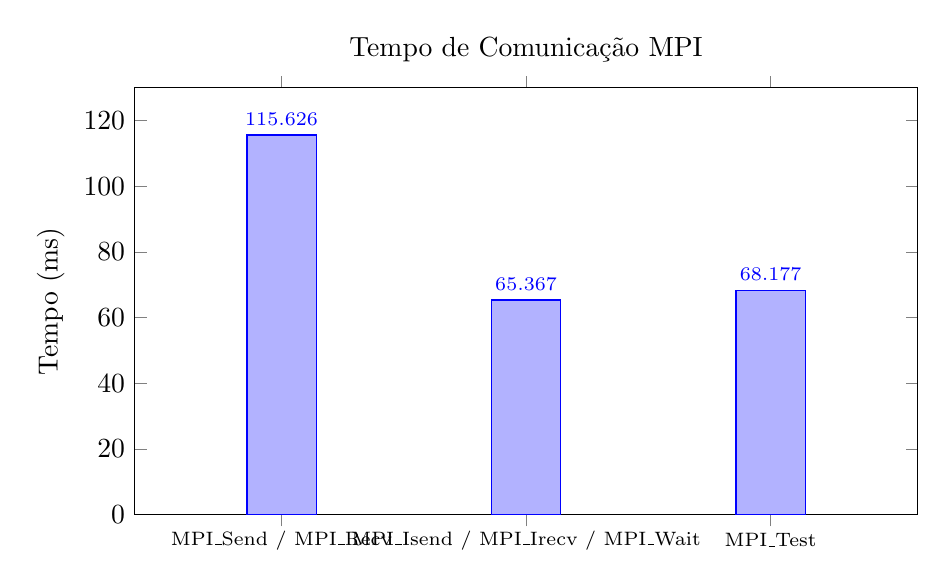
\begin{tikzpicture}
			\begin{axis}[
				title={Tempo de Comunica\c{c}\~{a}o MPI}, % Título do gráfico
				ybar,                                     % Define que é um gráfico de barras verticais
				enlarge x limits=0.3,                     % Aumenta o espaço nas extremidades do eixo x
				ylabel={Tempo (ms)},                      % Rótulo do eixo y (atualizado para milissegundos)
				xlabel={},    % Rótulo do eixo x
				symbolic x coords={                       % Define as coordenadas do eixo x simbolicamente
					MPI\_Send / MPI\_Recv,
					MPI\_Isend / MPI\_Irecv / MPI\_Wait,
					MPI\_Test
				},
				xtick=data,                               % Coloca os ticks do eixo x em cada barra
				nodes near coords,                        % Mostra o valor numérico perto do topo de cada barra
				every node near coord/.append style={     % Estiliza os números no topo das barras
					font=\scriptsize,                     % Define o tamanho da fonte dos números
					/pgf/number format/.cd,               % Acessa as configurações de formato de número
					fixed,                                % Usa formato de ponto fixo
					precision=3,                          % Define 3 casas decimais para os números (conforme dados de entrada)
					/tikz/.cd                             % Retorna ao caminho padrão do TikZ
				},
				nodes near coords align={above},          % Alinha os números acima das barras
				ymin=0,                                   % Eixo y começa em 0
				ymax=130,                                 % Valor máximo do eixo y (um pouco acima do maior valor: 115.626 ms)
				bar width=25pt,                           % Largura das barras
				xticklabel style={                        % Estiliza os rótulos do eixo x
					anchor=center,                       
					font=\scriptsize, 
					yshift=-5pt                     
				},
				width=0.95\textwidth,
				height=7cm,                      
				legend pos=north east,                    % Posição da legenda (se houver)
				]
				\addplot coordinates {
					(MPI\_Send / MPI\_Recv, 115.626)
					(MPI\_Isend / MPI\_Irecv / MPI\_Wait, 65.367)
					(MPI\_Test, 68.177)
				};
			\end{axis}
		\end{tikzpicture}
		\caption{Tempo de execução do programa usando tipos de comunicação diferentes em milissegundos.}
		\label{fig:mpi_communication_times_ms} 
		
	\end{figure}
	
	\section{Análise dos Resultados}
	
	\hspace{0.62cm}A Figura~\ref{fig:mpi_communication_times_ms} apresenta os tempos de execução medidos para as três versões implementadas da simulação de difusão de calor, utilizando diferentes estratégias de comunicação com MPI. Observa-se que a versão que utiliza \texttt{MPI\_Send/MPI\_Recv}, com comunicação bloqueante, apresentou o maior tempo de execução, aproximadamente \textbf{115,626 ms}. Isso ocorre devido ao comportamento bloqueante dessas funções, que força o processo a aguardar a conclusão de cada envio ou recebimento antes de prosseguir, resultando em períodos de inatividade (ociosos) e menor aproveitamento do processador.
	
	Em contrapartida, as versões que utilizam comunicação não bloqueante (\texttt{MPI\_Isend}/\texttt{MPI\_Irecv}) apresentaram desempenhos superiores. A versão intermediária, que utiliza \texttt{MPI\_Waitall} para aguardar a conclusão de todas as comunicações antes de iniciar o cálculo, apresentou um tempo de execução de aproximadamente \textbf{65,367 ms}, representando uma redução de cerca de \textbf{43,5\%} em relação à versão bloqueante. Isso evidencia que, mesmo sem explorar plenamente a sobreposição entre comunicação e computação, a simples adoção de operações não bloqueantes reduz significativamente o tempo de execução, ao evitar bloqueios desnecessários durante o envio e recebimento de mensagens.
	
	Por fim, a versão mais otimizada, que utiliza \texttt{MPI\_Test} para verificar dinamicamente a conclusão das comunicações de borda e iniciar o cálculo dos pontos internos enquanto a comunicação ainda está em andamento, apresentou um tempo de execução de \textbf{68,177 ms}. Embora esse valor seja ligeiramente superior ao obtido com \texttt{MPI\_Waitall}, ainda representa uma redução significativa em relação à versão bloqueante. A pequena diferença entre as versões com e sem sobreposição pode ser atribuída ao tamanho relativamente pequeno da malha processada ou ao custo associado à verificação contínua das operações com \texttt{MPI\_Test}, o que pode não ter proporcionado um ganho expressivo no cenário considerado.
	
	Além da redução do tempo de execução, foi possível observar o impacto positivo da sobreposição de comunicação e computação no \textbf{throughput} do programa, medido em milhões de operações de ponto flutuante por segundo (Mflops/s). A versão bloqueante apresentou um throughput de aproximadamente \textbf{43,0 Mflops/s}, enquanto as versões não bloqueantes atingiram \textbf{76,1 Mflops/s} (\texttt{MPI\_Isend}/\texttt{MPI\_Irecv}/\texttt{MPI\_Wait}) e \textbf{73,0 Mflops/s} (\texttt{MPI\_Test}), evidenciando um aumento significativo na eficiência computacional quando se reduz o tempo de espera na comunicação.
	
	Em síntese, os resultados demonstram claramente os benefícios da utilização de comunicações não bloqueantes em programas paralelos com MPI, tanto na redução do tempo de execução quanto no aumento do throughput. A versão com sobreposição total de comunicação e computação, embora não tenha superado em desempenho absoluto a versão com \texttt{MPI\_Waitall}, apresenta vantagens conceituais importantes, especialmente em cenários com maior carga computacional ou comunicações mais custosas, nos quais a sobreposição pode resultar em ganhos ainda mais expressivos.
	
	\section{Conclusão}
	
	\hspace{0.62cm}A realização desta atividade permitiu compreender, na prática, como diferentes estratégias de comunicação impactam o desempenho de aplicações paralelas. As versões que utilizam comunicação não bloqueante apresentaram tempos de execução inferiores à versão bloqueante, confirmando a eficiência da sobreposição entre comunicação e computação. Além disso, a versão com \texttt{MPI\_Test} mostrou-se vantajosa ao permitir o aproveitamento do tempo de espera para realizar cálculos, evidenciando a importância de técnicas que exploram a simultaneidade entre comunicação e processamento em sistemas distribuídos.	
	
	\end{document}
	
\end{document}
